\documentclass{standalone}
\usepackage{tikz}
\begin{document}
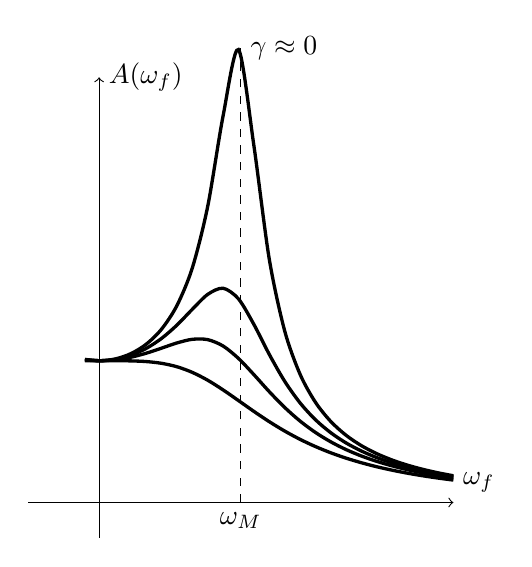
\begin{tikzpicture}[scale=1.8]
    \draw[->](-0.5,0)--(2.5,0)node[above right]{$\omega_f$};
    \draw[->](0,-0.25)--(0,3)node[right]{$A(\omega_f)$};

    
    \draw[very thick]plot[smooth, domain=-0.1:2.5](\x,{((1-(\x)^2)^2+2*(\x)^2)^-0.5});
    \draw[very thick]plot[smooth, domain=-0.1:2.5](\x,{((1-(\x)^2)^2+(\x)^2)^-0.5});
    \draw[very thick]plot[smooth, domain=-0.1:2.5](\x,{((1-(\x)^2)^2+0.5*(\x)^2)^-0.5});
    \draw[very thick]plot[smooth, domain=-0.1:2.5](\x,{((1-(\x)^2)^2+0.1*(\x)^2)^-0.5});


    \draw[dashed](1,0)node[below]{$\omega_M$}--(1,3.203)node[right]{$\gamma\approx0$};
\end{tikzpicture}
\end{document}